% Created by tikzDevice version 0.7.0 on 2015-09-11 16:22:41
% !TEX encoding = UTF-8 Unicode
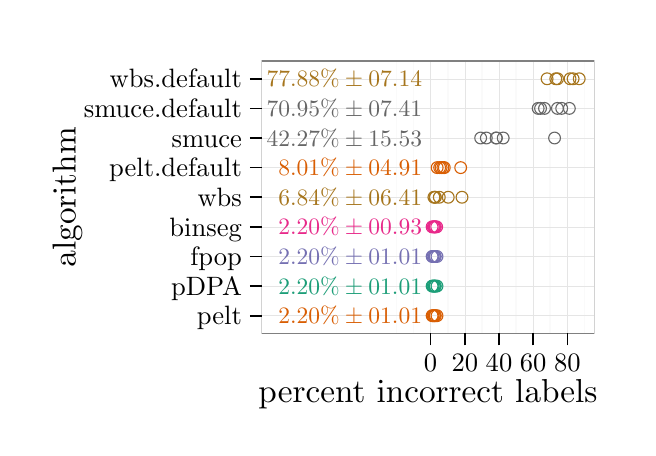
\begin{tikzpicture}[x=1pt,y=1pt]
\definecolor[named]{fillColor}{rgb}{1.00,1.00,1.00}
\path[use as bounding box,fill=fillColor,fill opacity=0.00] (0,0) rectangle (216.81,144.54);
\begin{scope}
\path[clip] (  0.00,  0.00) rectangle (216.81,144.54);
\definecolor[named]{drawColor}{rgb}{1.00,1.00,1.00}
\definecolor[named]{fillColor}{rgb}{1.00,1.00,1.00}

\path[draw=drawColor,line width= 0.6pt,line join=round,line cap=round,fill=fillColor] ( -0.00,  0.00) rectangle (216.81,144.54);
\end{scope}
\begin{scope}
\path[clip] ( 84.53, 34.03) rectangle (204.76,132.50);
\definecolor[named]{fillColor}{rgb}{1.00,1.00,1.00}

\path[fill=fillColor] ( 84.53, 34.03) rectangle (204.77,132.50);
\definecolor[named]{drawColor}{rgb}{0.98,0.98,0.98}

\path[draw=drawColor,line width= 0.6pt,line join=round] (133.25, 34.03) --
	(133.25,132.50);

\path[draw=drawColor,line width= 0.6pt,line join=round] (139.42, 34.03) --
	(139.42,132.50);

\path[draw=drawColor,line width= 0.6pt,line join=round] (151.78, 34.03) --
	(151.78,132.50);

\path[draw=drawColor,line width= 0.6pt,line join=round] (164.14, 34.03) --
	(164.14,132.50);

\path[draw=drawColor,line width= 0.6pt,line join=round] (176.50, 34.03) --
	(176.50,132.50);

\path[draw=drawColor,line width= 0.6pt,line join=round] (188.85, 34.03) --
	(188.85,132.50);

\path[draw=drawColor,line width= 0.6pt,line join=round] (201.21, 34.03) --
	(201.21,132.50);
\definecolor[named]{drawColor}{rgb}{0.90,0.90,0.90}

\path[draw=drawColor,line width= 0.2pt,line join=round] ( 84.53, 40.46) --
	(204.76, 40.46);

\path[draw=drawColor,line width= 0.2pt,line join=round] ( 84.53, 51.16) --
	(204.76, 51.16);

\path[draw=drawColor,line width= 0.2pt,line join=round] ( 84.53, 61.86) --
	(204.76, 61.86);

\path[draw=drawColor,line width= 0.2pt,line join=round] ( 84.53, 72.56) --
	(204.76, 72.56);

\path[draw=drawColor,line width= 0.2pt,line join=round] ( 84.53, 83.26) --
	(204.76, 83.26);

\path[draw=drawColor,line width= 0.2pt,line join=round] ( 84.53, 93.97) --
	(204.76, 93.97);

\path[draw=drawColor,line width= 0.2pt,line join=round] ( 84.53,104.67) --
	(204.76,104.67);

\path[draw=drawColor,line width= 0.2pt,line join=round] ( 84.53,115.37) --
	(204.76,115.37);

\path[draw=drawColor,line width= 0.2pt,line join=round] ( 84.53,126.07) --
	(204.76,126.07);

\path[draw=drawColor,line width= 0.2pt,line join=round] (145.60, 34.03) --
	(145.60,132.50);

\path[draw=drawColor,line width= 0.2pt,line join=round] (157.96, 34.03) --
	(157.96,132.50);

\path[draw=drawColor,line width= 0.2pt,line join=round] (170.32, 34.03) --
	(170.32,132.50);

\path[draw=drawColor,line width= 0.2pt,line join=round] (182.67, 34.03) --
	(182.67,132.50);

\path[draw=drawColor,line width= 0.2pt,line join=round] (195.03, 34.03) --
	(195.03,132.50);
\definecolor[named]{drawColor}{rgb}{0.85,0.37,0.01}

\node[text=drawColor,anchor=base east,inner sep=0pt, outer sep=0pt, scale=  0.85] at (142.51, 37.53) {$2.20\% \pm 01.01$};
\definecolor[named]{drawColor}{rgb}{0.11,0.62,0.47}

\node[text=drawColor,anchor=base east,inner sep=0pt, outer sep=0pt, scale=  0.85] at (142.51, 48.23) {$2.20\% \pm 01.01$};
\definecolor[named]{drawColor}{rgb}{0.46,0.44,0.70}

\node[text=drawColor,anchor=base east,inner sep=0pt, outer sep=0pt, scale=  0.85] at (142.51, 58.93) {$2.20\% \pm 01.01$};
\definecolor[named]{drawColor}{rgb}{0.91,0.16,0.54}

\node[text=drawColor,anchor=base east,inner sep=0pt, outer sep=0pt, scale=  0.85] at (142.51, 69.63) {$2.20\% \pm 00.93$};
\definecolor[named]{drawColor}{rgb}{0.65,0.46,0.11}

\node[text=drawColor,anchor=base east,inner sep=0pt, outer sep=0pt, scale=  0.85] at (142.51, 80.34) {$6.84\% \pm 06.41$};
\definecolor[named]{drawColor}{rgb}{0.85,0.37,0.01}

\node[text=drawColor,anchor=base east,inner sep=0pt, outer sep=0pt, scale=  0.85] at (142.51, 91.04) {$8.01\% \pm 04.91$};
\definecolor[named]{drawColor}{rgb}{0.40,0.40,0.40}

\node[text=drawColor,anchor=base east,inner sep=0pt, outer sep=0pt, scale=  0.85] at (142.51,101.74) {$42.27\% \pm 15.53$};

\node[text=drawColor,anchor=base east,inner sep=0pt, outer sep=0pt, scale=  0.85] at (142.51,112.44) {$70.95\% \pm 07.41$};
\definecolor[named]{drawColor}{rgb}{0.65,0.46,0.11}

\node[text=drawColor,anchor=base east,inner sep=0pt, outer sep=0pt, scale=  0.85] at (142.51,123.15) {$77.88\% \pm 07.14$};
\definecolor[named]{drawColor}{rgb}{0.85,0.37,0.01}

\path[draw=drawColor,line width= 0.4pt,line join=round,line cap=round] (146.91, 40.46) circle (  2.13);

\path[draw=drawColor,line width= 0.4pt,line join=round,line cap=round] (147.32, 40.46) circle (  2.13);

\path[draw=drawColor,line width= 0.4pt,line join=round,line cap=round] (146.14, 40.46) circle (  2.13);

\path[draw=drawColor,line width= 0.4pt,line join=round,line cap=round] (147.01, 40.46) circle (  2.13);

\path[draw=drawColor,line width= 0.4pt,line join=round,line cap=round] (146.47, 40.46) circle (  2.13);

\path[draw=drawColor,line width= 0.4pt,line join=round,line cap=round] (147.91, 40.46) circle (  2.13);
\definecolor[named]{drawColor}{rgb}{0.11,0.62,0.47}

\path[draw=drawColor,line width= 0.4pt,line join=round,line cap=round] (146.91, 51.16) circle (  2.13);

\path[draw=drawColor,line width= 0.4pt,line join=round,line cap=round] (147.32, 51.16) circle (  2.13);

\path[draw=drawColor,line width= 0.4pt,line join=round,line cap=round] (146.14, 51.16) circle (  2.13);

\path[draw=drawColor,line width= 0.4pt,line join=round,line cap=round] (147.01, 51.16) circle (  2.13);

\path[draw=drawColor,line width= 0.4pt,line join=round,line cap=round] (146.47, 51.16) circle (  2.13);

\path[draw=drawColor,line width= 0.4pt,line join=round,line cap=round] (147.91, 51.16) circle (  2.13);
\definecolor[named]{drawColor}{rgb}{0.46,0.44,0.70}

\path[draw=drawColor,line width= 0.4pt,line join=round,line cap=round] (146.91, 61.86) circle (  2.13);

\path[draw=drawColor,line width= 0.4pt,line join=round,line cap=round] (147.32, 61.86) circle (  2.13);

\path[draw=drawColor,line width= 0.4pt,line join=round,line cap=round] (146.14, 61.86) circle (  2.13);

\path[draw=drawColor,line width= 0.4pt,line join=round,line cap=round] (147.01, 61.86) circle (  2.13);

\path[draw=drawColor,line width= 0.4pt,line join=round,line cap=round] (146.47, 61.86) circle (  2.13);

\path[draw=drawColor,line width= 0.4pt,line join=round,line cap=round] (147.91, 61.86) circle (  2.13);
\definecolor[named]{drawColor}{rgb}{0.91,0.16,0.54}

\path[draw=drawColor,line width= 0.4pt,line join=round,line cap=round] (146.91, 72.56) circle (  2.13);

\path[draw=drawColor,line width= 0.4pt,line join=round,line cap=round] (147.32, 72.56) circle (  2.13);

\path[draw=drawColor,line width= 0.4pt,line join=round,line cap=round] (146.14, 72.56) circle (  2.13);

\path[draw=drawColor,line width= 0.4pt,line join=round,line cap=round] (147.01, 72.56) circle (  2.13);

\path[draw=drawColor,line width= 0.4pt,line join=round,line cap=round] (146.58, 72.56) circle (  2.13);

\path[draw=drawColor,line width= 0.4pt,line join=round,line cap=round] (147.80, 72.56) circle (  2.13);
\definecolor[named]{drawColor}{rgb}{0.65,0.46,0.11}

\path[draw=drawColor,line width= 0.4pt,line join=round,line cap=round] (156.94, 83.26) circle (  2.13);

\path[draw=drawColor,line width= 0.4pt,line join=round,line cap=round] (147.32, 83.26) circle (  2.13);

\path[draw=drawColor,line width= 0.4pt,line join=round,line cap=round] (146.79, 83.26) circle (  2.13);

\path[draw=drawColor,line width= 0.4pt,line join=round,line cap=round] (147.23, 83.26) circle (  2.13);

\path[draw=drawColor,line width= 0.4pt,line join=round,line cap=round] (148.74, 83.26) circle (  2.13);

\path[draw=drawColor,line width= 0.4pt,line join=round,line cap=round] (151.97, 83.26) circle (  2.13);
\definecolor[named]{drawColor}{rgb}{0.85,0.37,0.01}

\path[draw=drawColor,line width= 0.4pt,line join=round,line cap=round] (148.87, 93.97) circle (  2.13);

\path[draw=drawColor,line width= 0.4pt,line join=round,line cap=round] (150.55, 93.97) circle (  2.13);

\path[draw=drawColor,line width= 0.4pt,line join=round,line cap=round] (147.97, 93.97) circle (  2.13);

\path[draw=drawColor,line width= 0.4pt,line join=round,line cap=round] (149.40, 93.97) circle (  2.13);

\path[draw=drawColor,line width= 0.4pt,line join=round,line cap=round] (150.04, 93.97) circle (  2.13);

\path[draw=drawColor,line width= 0.4pt,line join=round,line cap=round] (156.47, 93.97) circle (  2.13);
\definecolor[named]{drawColor}{rgb}{0.40,0.40,0.40}

\path[draw=drawColor,line width= 0.4pt,line join=round,line cap=round] (190.39,104.67) circle (  2.13);

\path[draw=drawColor,line width= 0.4pt,line join=round,line cap=round] (163.69,104.67) circle (  2.13);

\path[draw=drawColor,line width= 0.4pt,line join=round,line cap=round] (169.28,104.67) circle (  2.13);

\path[draw=drawColor,line width= 0.4pt,line join=round,line cap=round] (169.38,104.67) circle (  2.13);

\path[draw=drawColor,line width= 0.4pt,line join=round,line cap=round] (165.73,104.67) circle (  2.13);

\path[draw=drawColor,line width= 0.4pt,line join=round,line cap=round] (171.83,104.67) circle (  2.13);

\path[draw=drawColor,line width= 0.4pt,line join=round,line cap=round] (195.73,115.37) circle (  2.13);

\path[draw=drawColor,line width= 0.4pt,line join=round,line cap=round] (184.46,115.37) circle (  2.13);

\path[draw=drawColor,line width= 0.4pt,line join=round,line cap=round] (192.97,115.37) circle (  2.13);

\path[draw=drawColor,line width= 0.4pt,line join=round,line cap=round] (191.43,115.37) circle (  2.13);

\path[draw=drawColor,line width= 0.4pt,line join=round,line cap=round] (185.32,115.37) circle (  2.13);

\path[draw=drawColor,line width= 0.4pt,line join=round,line cap=round] (186.76,115.37) circle (  2.13);
\definecolor[named]{drawColor}{rgb}{0.65,0.46,0.11}

\path[draw=drawColor,line width= 0.4pt,line join=round,line cap=round] (195.98,126.07) circle (  2.13);

\path[draw=drawColor,line width= 0.4pt,line join=round,line cap=round] (190.83,126.07) circle (  2.13);

\path[draw=drawColor,line width= 0.4pt,line join=round,line cap=round] (199.30,126.07) circle (  2.13);

\path[draw=drawColor,line width= 0.4pt,line join=round,line cap=round] (197.09,126.07) circle (  2.13);

\path[draw=drawColor,line width= 0.4pt,line join=round,line cap=round] (191.46,126.07) circle (  2.13);

\path[draw=drawColor,line width= 0.4pt,line join=round,line cap=round] (187.69,126.07) circle (  2.13);
\definecolor[named]{drawColor}{rgb}{0.50,0.50,0.50}

\path[draw=drawColor,line width= 0.6pt,line join=round,line cap=round] ( 84.53, 34.03) rectangle (204.77,132.50);
\end{scope}
\begin{scope}
\path[clip] (  0.00,  0.00) rectangle (216.81,144.54);
\definecolor[named]{drawColor}{rgb}{0.00,0.00,0.00}

\node[text=drawColor,anchor=base east,inner sep=0pt, outer sep=0pt, scale=  0.96] at ( 77.42, 37.15) {pelt};

\node[text=drawColor,anchor=base east,inner sep=0pt, outer sep=0pt, scale=  0.96] at ( 77.42, 47.85) {pDPA};

\node[text=drawColor,anchor=base east,inner sep=0pt, outer sep=0pt, scale=  0.96] at ( 77.42, 58.55) {fpop};

\node[text=drawColor,anchor=base east,inner sep=0pt, outer sep=0pt, scale=  0.96] at ( 77.42, 69.26) {binseg};

\node[text=drawColor,anchor=base east,inner sep=0pt, outer sep=0pt, scale=  0.96] at ( 77.42, 79.96) {wbs};

\node[text=drawColor,anchor=base east,inner sep=0pt, outer sep=0pt, scale=  0.96] at ( 77.42, 90.66) {pelt.default};

\node[text=drawColor,anchor=base east,inner sep=0pt, outer sep=0pt, scale=  0.96] at ( 77.42,101.36) {smuce};

\node[text=drawColor,anchor=base east,inner sep=0pt, outer sep=0pt, scale=  0.96] at ( 77.42,112.07) {smuce.default};

\node[text=drawColor,anchor=base east,inner sep=0pt, outer sep=0pt, scale=  0.96] at ( 77.42,122.77) {wbs.default};
\end{scope}
\begin{scope}
\path[clip] (  0.00,  0.00) rectangle (216.81,144.54);
\definecolor[named]{drawColor}{rgb}{0.00,0.00,0.00}

\path[draw=drawColor,line width= 0.6pt,line join=round] ( 80.26, 40.46) --
	( 84.53, 40.46);

\path[draw=drawColor,line width= 0.6pt,line join=round] ( 80.26, 51.16) --
	( 84.53, 51.16);

\path[draw=drawColor,line width= 0.6pt,line join=round] ( 80.26, 61.86) --
	( 84.53, 61.86);

\path[draw=drawColor,line width= 0.6pt,line join=round] ( 80.26, 72.56) --
	( 84.53, 72.56);

\path[draw=drawColor,line width= 0.6pt,line join=round] ( 80.26, 83.26) --
	( 84.53, 83.26);

\path[draw=drawColor,line width= 0.6pt,line join=round] ( 80.26, 93.97) --
	( 84.53, 93.97);

\path[draw=drawColor,line width= 0.6pt,line join=round] ( 80.26,104.67) --
	( 84.53,104.67);

\path[draw=drawColor,line width= 0.6pt,line join=round] ( 80.26,115.37) --
	( 84.53,115.37);

\path[draw=drawColor,line width= 0.6pt,line join=round] ( 80.26,126.07) --
	( 84.53,126.07);
\end{scope}
\begin{scope}
\path[clip] (  0.00,  0.00) rectangle (216.81,144.54);
\definecolor[named]{drawColor}{rgb}{0.00,0.00,0.00}

\path[draw=drawColor,line width= 0.6pt,line join=round] (145.60, 29.77) --
	(145.60, 34.03);

\path[draw=drawColor,line width= 0.6pt,line join=round] (157.96, 29.77) --
	(157.96, 34.03);

\path[draw=drawColor,line width= 0.6pt,line join=round] (170.32, 29.77) --
	(170.32, 34.03);

\path[draw=drawColor,line width= 0.6pt,line join=round] (182.67, 29.77) --
	(182.67, 34.03);

\path[draw=drawColor,line width= 0.6pt,line join=round] (195.03, 29.77) --
	(195.03, 34.03);
\end{scope}
\begin{scope}
\path[clip] (  0.00,  0.00) rectangle (216.81,144.54);
\definecolor[named]{drawColor}{rgb}{0.00,0.00,0.00}

\node[text=drawColor,anchor=base,inner sep=0pt, outer sep=0pt, scale=  0.96] at (145.60, 20.31) {0};

\node[text=drawColor,anchor=base,inner sep=0pt, outer sep=0pt, scale=  0.96] at (157.96, 20.31) {20};

\node[text=drawColor,anchor=base,inner sep=0pt, outer sep=0pt, scale=  0.96] at (170.32, 20.31) {40};

\node[text=drawColor,anchor=base,inner sep=0pt, outer sep=0pt, scale=  0.96] at (182.67, 20.31) {60};

\node[text=drawColor,anchor=base,inner sep=0pt, outer sep=0pt, scale=  0.96] at (195.03, 20.31) {80};
\end{scope}
\begin{scope}
\path[clip] (  0.00,  0.00) rectangle (216.81,144.54);
\definecolor[named]{drawColor}{rgb}{0.00,0.00,0.00}

\node[text=drawColor,anchor=base,inner sep=0pt, outer sep=0pt, scale=  1.20] at (144.65,  9.03) {percent incorrect labels};
\end{scope}
\begin{scope}
\path[clip] (  0.00,  0.00) rectangle (216.81,144.54);
\definecolor[named]{drawColor}{rgb}{0.00,0.00,0.00}

\node[text=drawColor,rotate= 90.00,anchor=base,inner sep=0pt, outer sep=0pt, scale=  1.20] at ( 17.30, 83.26) {algorithm};
\end{scope}
\end{tikzpicture}
